\chapter{Background and Related Works in the Field}
    \section{Environmental Storytelling}
        \subsection{Definition of Environmental Storytelling} Define "environmental narration" (storytelling through space, atmosphere, implicit cues).
        \subsection{Existing Methods in Different Mediums} Discuss existing techniques in games, film, sound art, and literature (e.g., sound design, level design, environmental puzzles, use of acoustics).
        \subsection{Auditory Environmental Storytelling} Give an example from the Game Return of the Obra Dinn. 
    \section{Room Acoustics}
        \emph{"Sound is something most people take for granted. Our environment is full of noises, which we have been exposed to from before birth. What is sound, how does it propagate and how can it be quantified\cite{Blank}?"}\par 

        The purpose of this subchapter is to introduce fundamental knowledge ground for room acoustics and describe the usage of room impulse responses in the Embracing Sphere context.\par
        \subsection{Definitions for Room Acoustics}
            Sound is simply a mechanical disturbance of the medium. Medium in that context may be air, solid, liquid or other gas matters. Dependent on the mediums state, the sound can be propagated and while this propagation happens it interacts with physical objects and other sound waves. In room acoustics the interactions of the sound with the medium, basically can be listed as refraction, absorption, reflection and interference. Psychoacoustics is the study how humans perceive sound after all these interactions with the medium\cite{Blank}.\par

            The heard sound, is the result of all these complex physical interactions in the place our ears are located.\par

            When sound moves through a room, its behavior is shaped by how it interacts with surfaces, mainly through absorption and reflection. Sound reflection occurs when sound waves hit a hard boundary and bounce back into space. In contrast, sound absorption is when a material takes in the sound's energy, which is converted into small amounts of heat through internal friction, reducing the amount of sound that reflects\cite{Blank}. For example, a wooden surface absorbs more sound than a rough concrete one. These interactions, along with others like refraction and interference, collectively determine the acoustic character of a room.\par

            These interactions do not occur in isolation. They collectively define the complex behavior of sound waves and their propagation within the room. Each time the sound interacts with a surface in the room it loses some of its energy due to absorption and reflection. The time that it takes for sound at a given time to die away in a room is called the reverberation time.\par

            Reverberation time is an important aspect of sound behavior in a room. Mentioned different absorption coefficient values in different materials and frequencies shapes the perception of the room. If the sound dies away very quickly, we perceive the room as being “dead” or if the sound dies away very slowly, we perceive the room as being “live”. To calculate reverberation times there is a simple formula known as the “Sabine formula”, named after its developer Wallace Clement Sabine\cite{Blank}.\par 
            $$RT_{60} = \frac{0.161 \cdot V}{A}$$
            \begin{itemize}
                \item RT60: This is the reverberation time in seconds. It's defined as the time it takes for the sound pressure level in a room to decrease by 60 decibels (dB) after the sound source has stopped.
                \item 0.161: This is a constant. Its units are seconds per meter (s/m). This constant is derived empirically and is based on the speed of sound in air at a typical room temperature.
                \item V: This represents the volume of the room in cubic meters. Calculated by multiplying the length, width, and height of the room.
                \item A: This is the total sound absorption of the room in Sabins. It's calculated by summing the absorption of all surfaces in the room. The absorption of each surface is found by multiplying its surface area in square meters by its sound absorption coefficient at a specific frequency.
            \end{itemize}

            According to the Sabine formula, reverberation time depends on the volume, surface area, and the average absorption coefficient in the room. However, the absorption coefficients of real materials are not constant with frequency. This difference in absorption strength in different frequencies changes heard timbre of the room as the sound in the room decays away. Apart from being useful, Sabine formula has assumptions for speed of sound and static response of the reflective materials in the room. To more accurately measure reverberation time, another method introduced in 1964 by M. R. Schroeder called room impulse response capturing\cite{Blank}.\par

            The method uses tone bursts (or filtered pistol shots) to excite the enclosure(room). The captured smooth decay curves resulting from the new method improve the accuracy of reverberation time measurements and facilitate the detection of non-exponential decays\cite{Blank}.\par

            These impulse response recordings later can be used to reconstruct a virtual environment with the same reverberation curves as captured room with a mathematical operation called convolution. An anechoic(no reflections) sound is convolved with an RIR and this mathematical process applies the room's acoustic snapshot to the sound. The convolution effectively embeds the reflections and reverberation captured in the RIR to the original sound.
        \subsection{Room Impulse Response Measurement Methods} Overview of RIR measurement techniques.
        \subsection{Convolution in Math and Digital Audio} Explain Convolution operation and usage in audio-visual content.
        \subsection{Room Acoustics in Sound Art} Explain Alvin Lucier - "I Am Sitting in a Room" Process-based art, using the room's acoustics as both medium and subject, the iterative feedback loop revealing resonant frequencies.
    \section{Haptics and Perception}
        \subsection{Overview of Haptics}
            The somatic system can be subdivided into three elements: kinesthetic, visceral, and cutaneous. Kinesthetic sensation uses signals from proprioceptors in the joints, muscles, and tendons to provide feedback to the brain on the position and forces within segments. Similarly, visceral sensation uses receptors in the abdomen. Cutaneous sensation consists of a combined response of four types of nerve endings in the skin\cite{Blank}. The haptic system uses sensory information derived from mechanoreceptors embedded in the skin, muscles, tendons and joints\cite{Blank}.\par

            Haptic interaction can be stimulated by different devices but such as thermal feedback and electro-vibration are outside the scope of this study thus a vibrotactile device chosen for this research purpose. These vibrotactile devices are similar to those of loudspeakers and voice coil actuators\cite{Blank}, allowing for conventional audio recording practices viable on haptic feedback content creation.\par

            \begin{figure}[H]
                \centering
                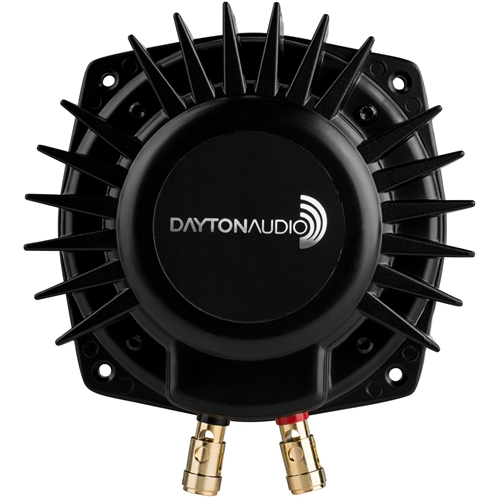
\includegraphics[width=0.4\textwidth]{images/vibrotactile_bass-shaker.jpg}
                \caption{Voice coil actuator, vibrotactile device, Dayton Audio BST-1.}
                \label{fig:VCA}
            \end{figure}

            The sensory system is a network that enables your body to receive information from the environment and its own internal state, converting stimuli into signals for the brain to process. Human sensory system doesn't just process this sensory information as a single stream; it organizes it to answer fundamental questions about the environment\cite{Blank}. Research in sensory neuroscience suggests a fundamental distinction in how the brain processes sensory information framed as "what" an object(disturbance) is versus "where" it is located.\par

            How do you feel the difference between rough stone, resonant wood, or soft earth? This relates directly to identifying the "what" of the surrounding environment. The "where" pathway provides spatial information, helping us understand the location of a stimulus in relation to our body and within the environment. The location of a distant explosion felt through the floor, or the feeling of being in a small, enclosed space versus an open one? This is related to identifying "where" information.\par

            Within the study that explores environmental storytelling through audio-tactile stimulation, we can extend this framework with a third component, "how". This component can include "cause and effect" relation into our sensory perception and cognition. Where "what" and "where" components answer material and spatial questions, "how" components can answer temporal questions derived from the first two components. Focusing on a more interactive concept of "event" rather than a static stimulation characteristics.\par

            This "what, where and how" taxonomy provides a conceptual tool for environmental storytelling, thus embedding temporal relations into the environment, moving beyond simple rumbles to convey specific information about an environment's materials, spatial layouts and past/ongoing events.\par

            \begin{figure}[H]
                \centering
                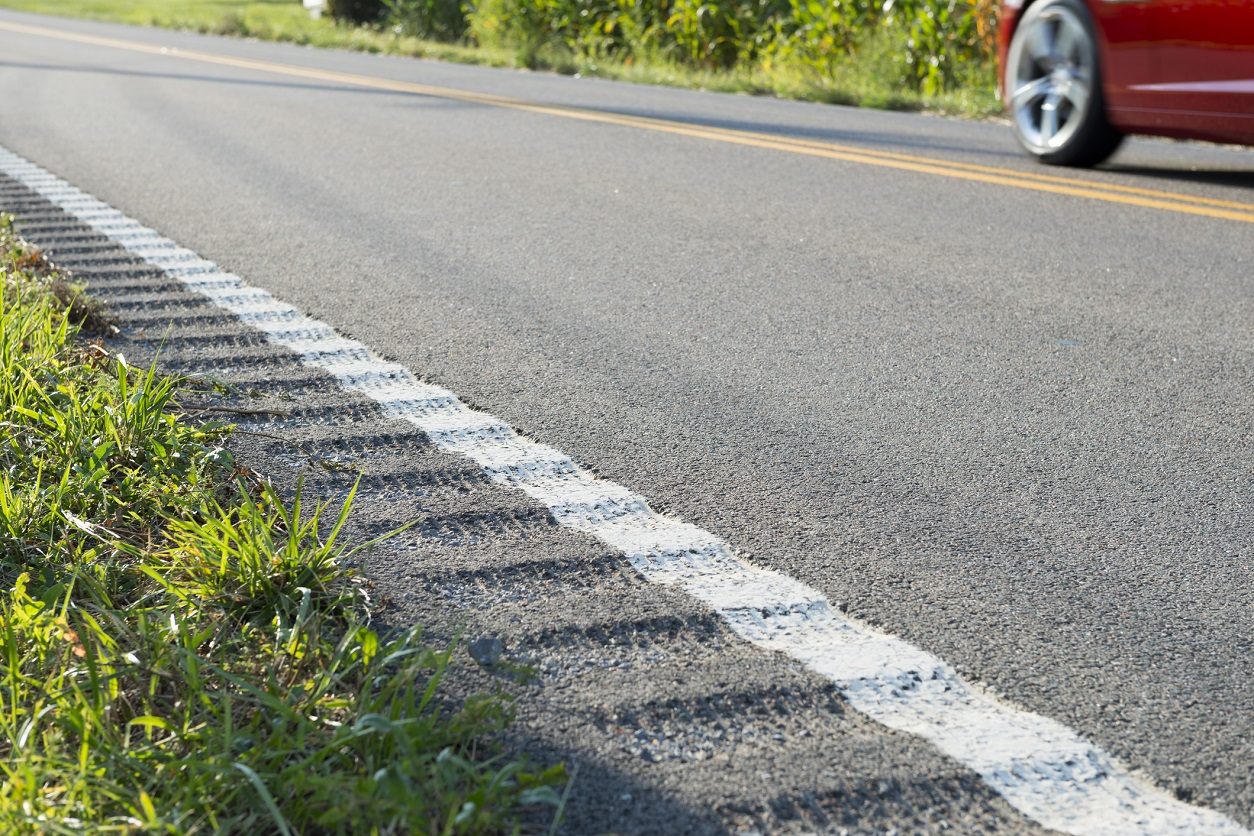
\includegraphics[width=0.8\textwidth]{images/rumble_strips.jpg}
                \caption{A visual shows road rumble strips.}
                \label{fig:RUMBLE_STRIP}
            \end{figure}

            As shown in the \ref{fig:RUMBLE_STRIP} rumble strips designed to alert drivers by creating vibrations and noise when a vehicle goes out from its intended lane or crosses the edge of the road. Stimulation from a rumble strip side of the road not just indicating physical position or a road surface information, it's an immediate warning.\par

            The sensation isn't a random patch of bad road; it's a deliberately engineered, rhythmic pattern. This pattern connects the what (the ribbed texture) and the where (the edge of the lane) to create a temporal meaning: "You are currently in the process of making a mistake." The "how" pathway interprets this sequence as a cause-and-effect event, because you are drifting, you are feeling this vibration. In a structured narrative context, this type of haptic stimulation can be utilized for environmental storytelling.\par

            \subsection{Human Tactile Perception} Briefly cover human tactile perception (how we sense texture, vibration, impact).
        \subsection{Usage} Examples of haptics in HCI, VR/AR, accessibility, and gaming.
    \section{Audio-Tactile Interaction}
        \subsection{Definition of Audio-Tactile Multi-Modal Interaction} Define audio-tactility and explain differences from other multi-modal systems.
        \subsection{Usage of Audio-Tactility in Media} Examples of systems or experiences integrating audio and haptics.